% Ubah kalimat sesuai dengan judul dari bab ini
\chapter{DESAIN DAN IMPLEMENTASI}

% Ubah konten-konten berikut sesuai dengan yang ingin diisi pada bab ini
\section{Deskripsi Sistem}

Sistem yang dikembangkan dalam kerja praktik ini adalah sebuah kerangka kerja \textit{fault tolerance} untuk pemrosesan citra medis, khususnya MRI otak. Sistem ini dirancang untuk melakukan mitigasi dampak negatif dari artefak gerak (\textit{motion artifacts}) sebelum citra diproses lebih lanjut oleh sistem lanjutan \textit{image captioning}. Secara garis besar, sistem terdiri dari tiga komponen utama yang saling terintegrasi:

\begin{enumerate}[nolistsep]
	\item \textbf{Modul simulasi data} yang bertugas untuk menghasilkan dataset sintetis untuk menyimulasikan artefak gerak yang terjadi di dunia nyata.
	
	\item \textbf{Modul klasifikasi artefak} yang bertugas mendeteksi jenis artefak gerak dengan empat kelas klasifikasi yaitu translasi horizontal, translasi vertikal, rotasi, dan gambar bersih pada citra.
	
	\item \textbf{Modul koreksi citra} yang bertugas merekonstruksi citra dengan artefak menjadi citra bersih.   
\end{enumerate}

\subsection{Desain Pembuatan Dataset Simulasi}

Untuk melatih model koreksi citra dengan Pix2Pix, diperlukan pasangan data citra bersih dan artefak. Sistem ini menggunakan pendekatan simulasi berbasis domain frekuensi (\textit{k-space}) untuk melakukan simulasi artefak gerak sesuai dengan kondisi pada dunia nyata. Proses pembuatan dataset latih ditunjukkan pada Gambar \ref{fig:flowchart-dataset}.

\begin{figure}[H]
	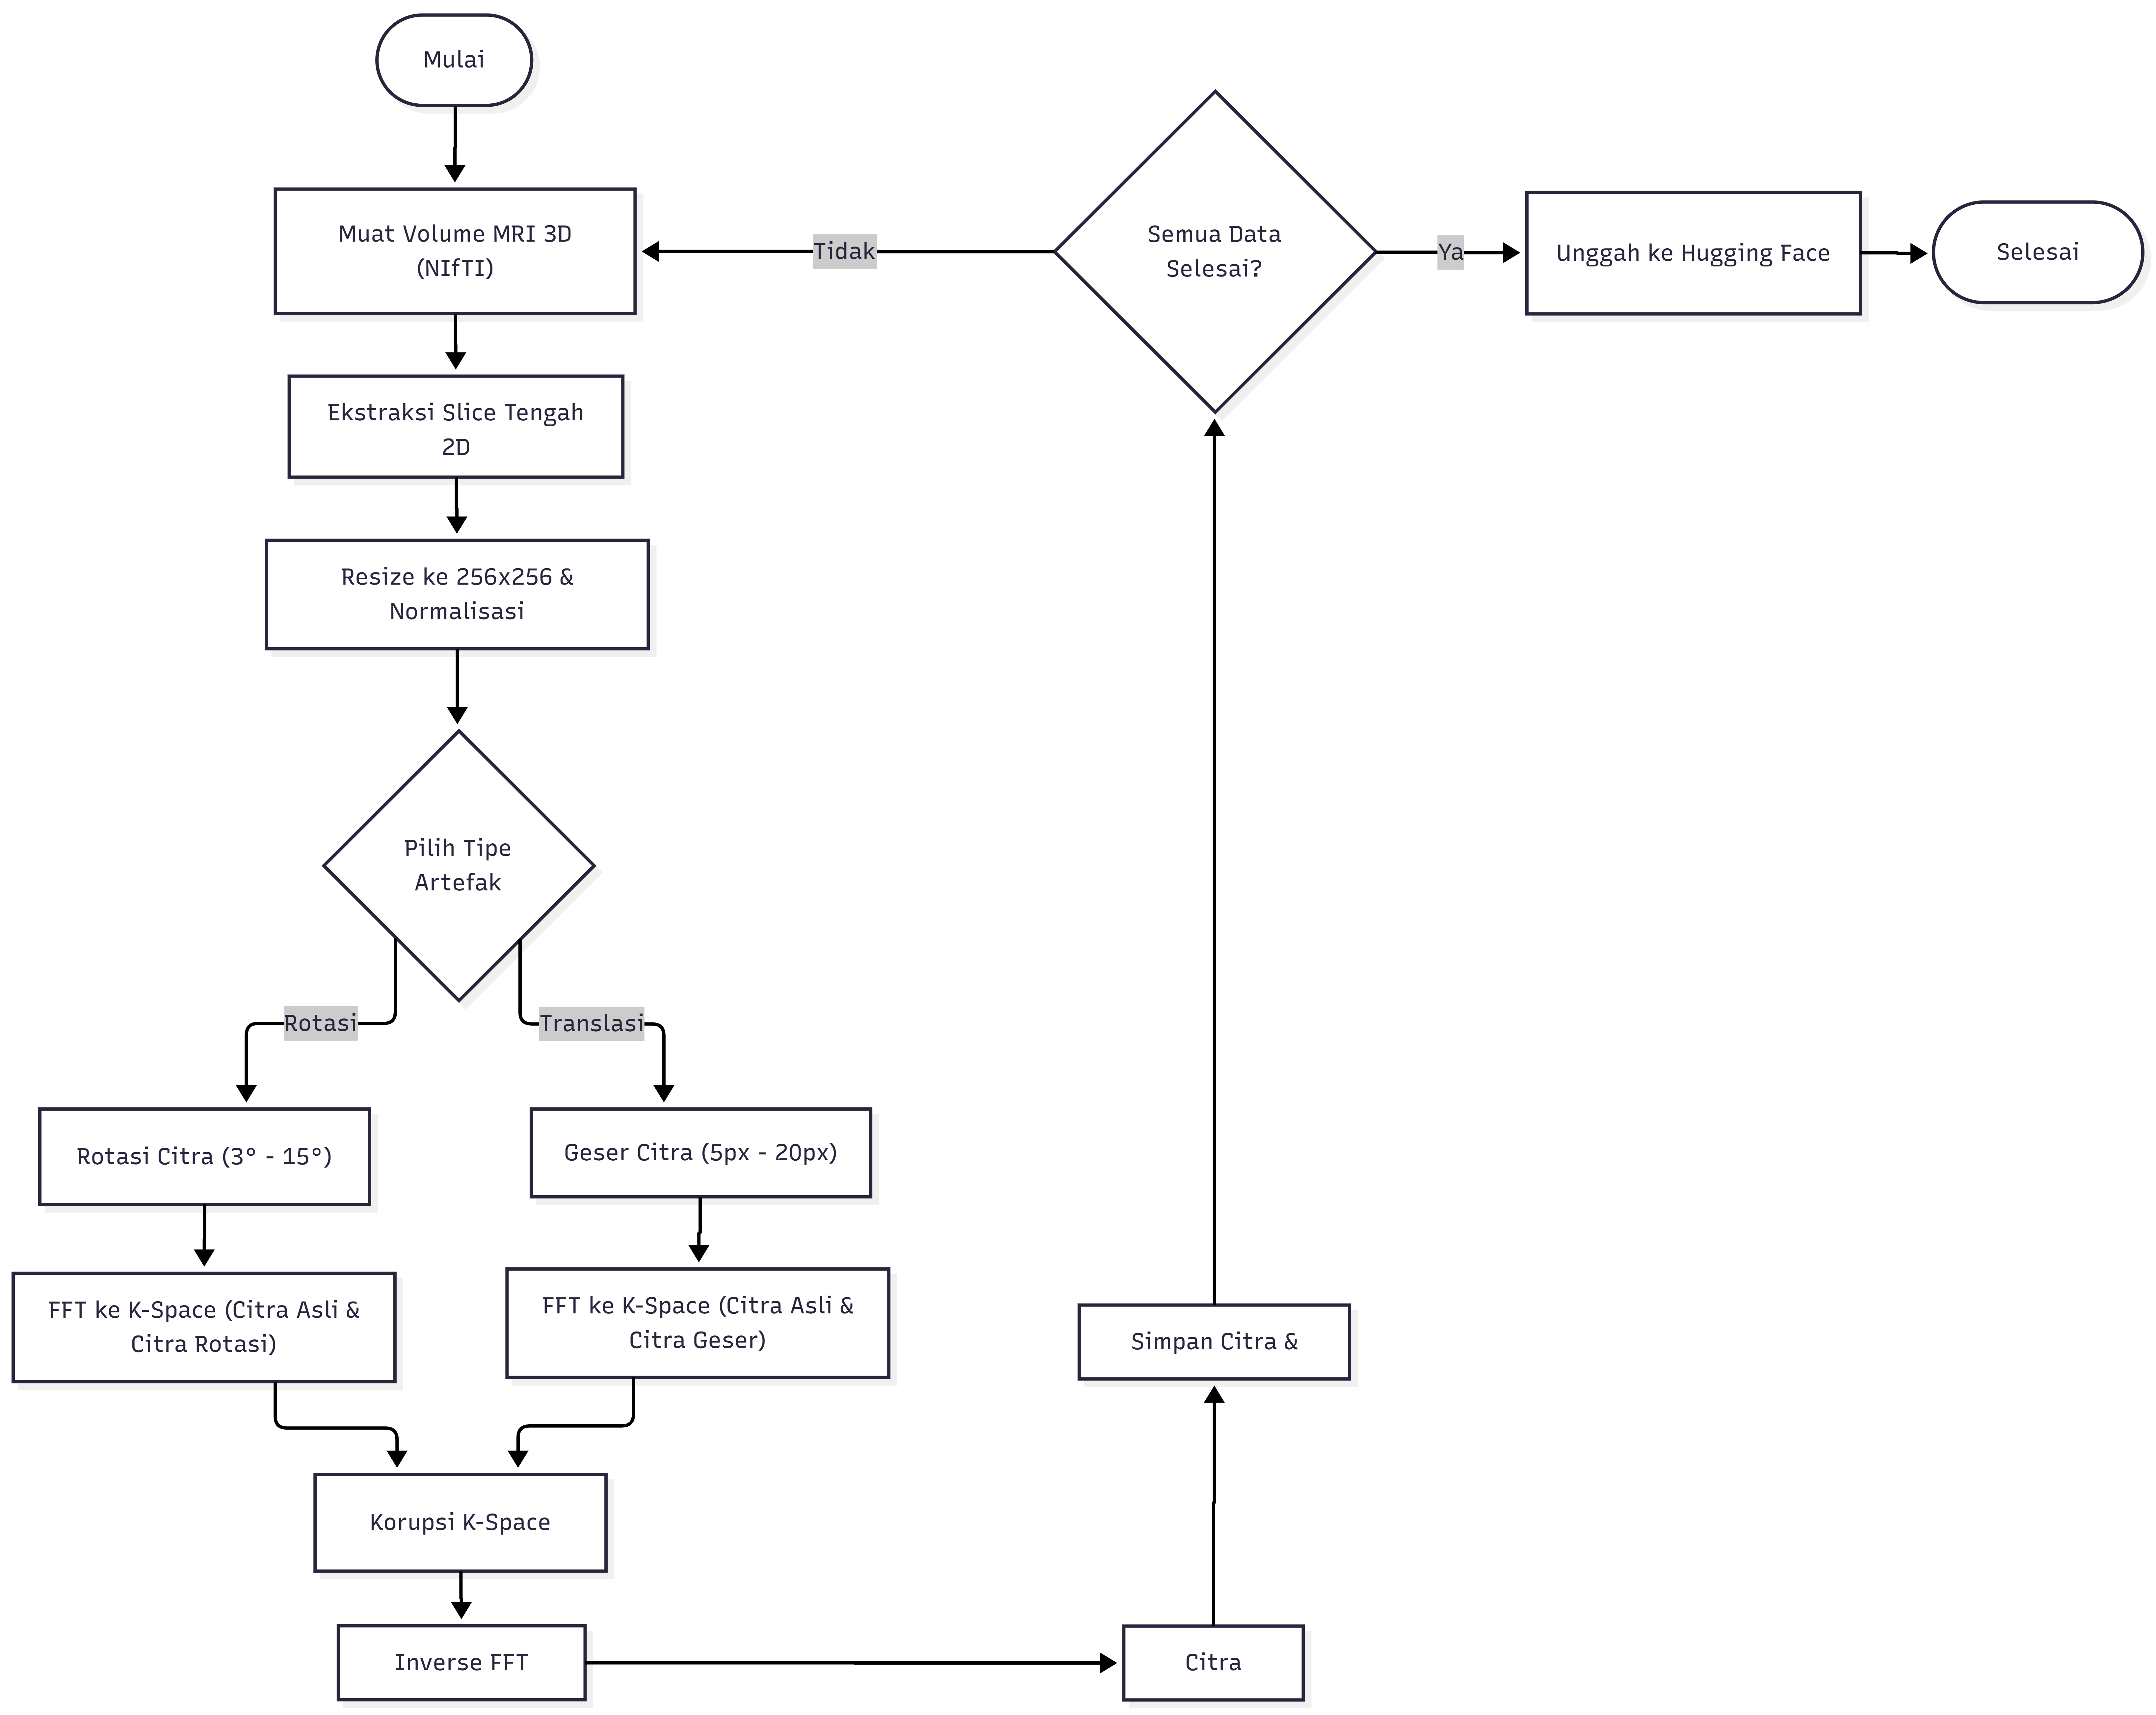
\includegraphics[width=\linewidth]{gambar/flowchart-dataset.png}
	\caption{Diagram Alur Pembuatan Dataset}
	\label{fig:flowchart-dataset}
\end{figure}

Secara umum, proses simulasi artefak terdiri dari tiga bagian, yaitu:

\begin{enumerate}[nolistsep]
	
	\item Transformasi citra bersih ke \textit{k-space} domain frekuensi menggunakan \textit{Fast Fourier Transform} (FFT).
	
	\item Simulasi artefak dengan menggabungkan (\textit{splicing}) garis-garis frekuensi dari citra diam dan citra yang dilakukan translasi atau rotasi. Hal ini meniru inkonsistensi fase yang terjadi ketika pasien bergerak selama pemindaian MRI.
	
	\item Rekonstruksi citra dari data \textit{corrupt k-space} dikembalikan ke domain spasial menggunakan \textit{Inverse FFT} untuk menghasilkan artefak \textit{ghosting} dan \textit{streaking} yang realistis.
	
\end{enumerate}

\subsection{Desain Modul Klasifikasi Artefak}

Modul klasifikasi dirancang menggunakan pendekatan \textit{Transfer Learning} dari model \textit{pre-trained} untuk mengklasifikasikan empat kelas artefak citra, yaitu bersih, \textit{horizontal translation}, \textit{vertical translation}, dan rotasi. Proses klasifikasi secara detail dapat dilihat pada Gambar \ref{fig:flowchart-klasifikasi}.

\begin{figure}[H]
	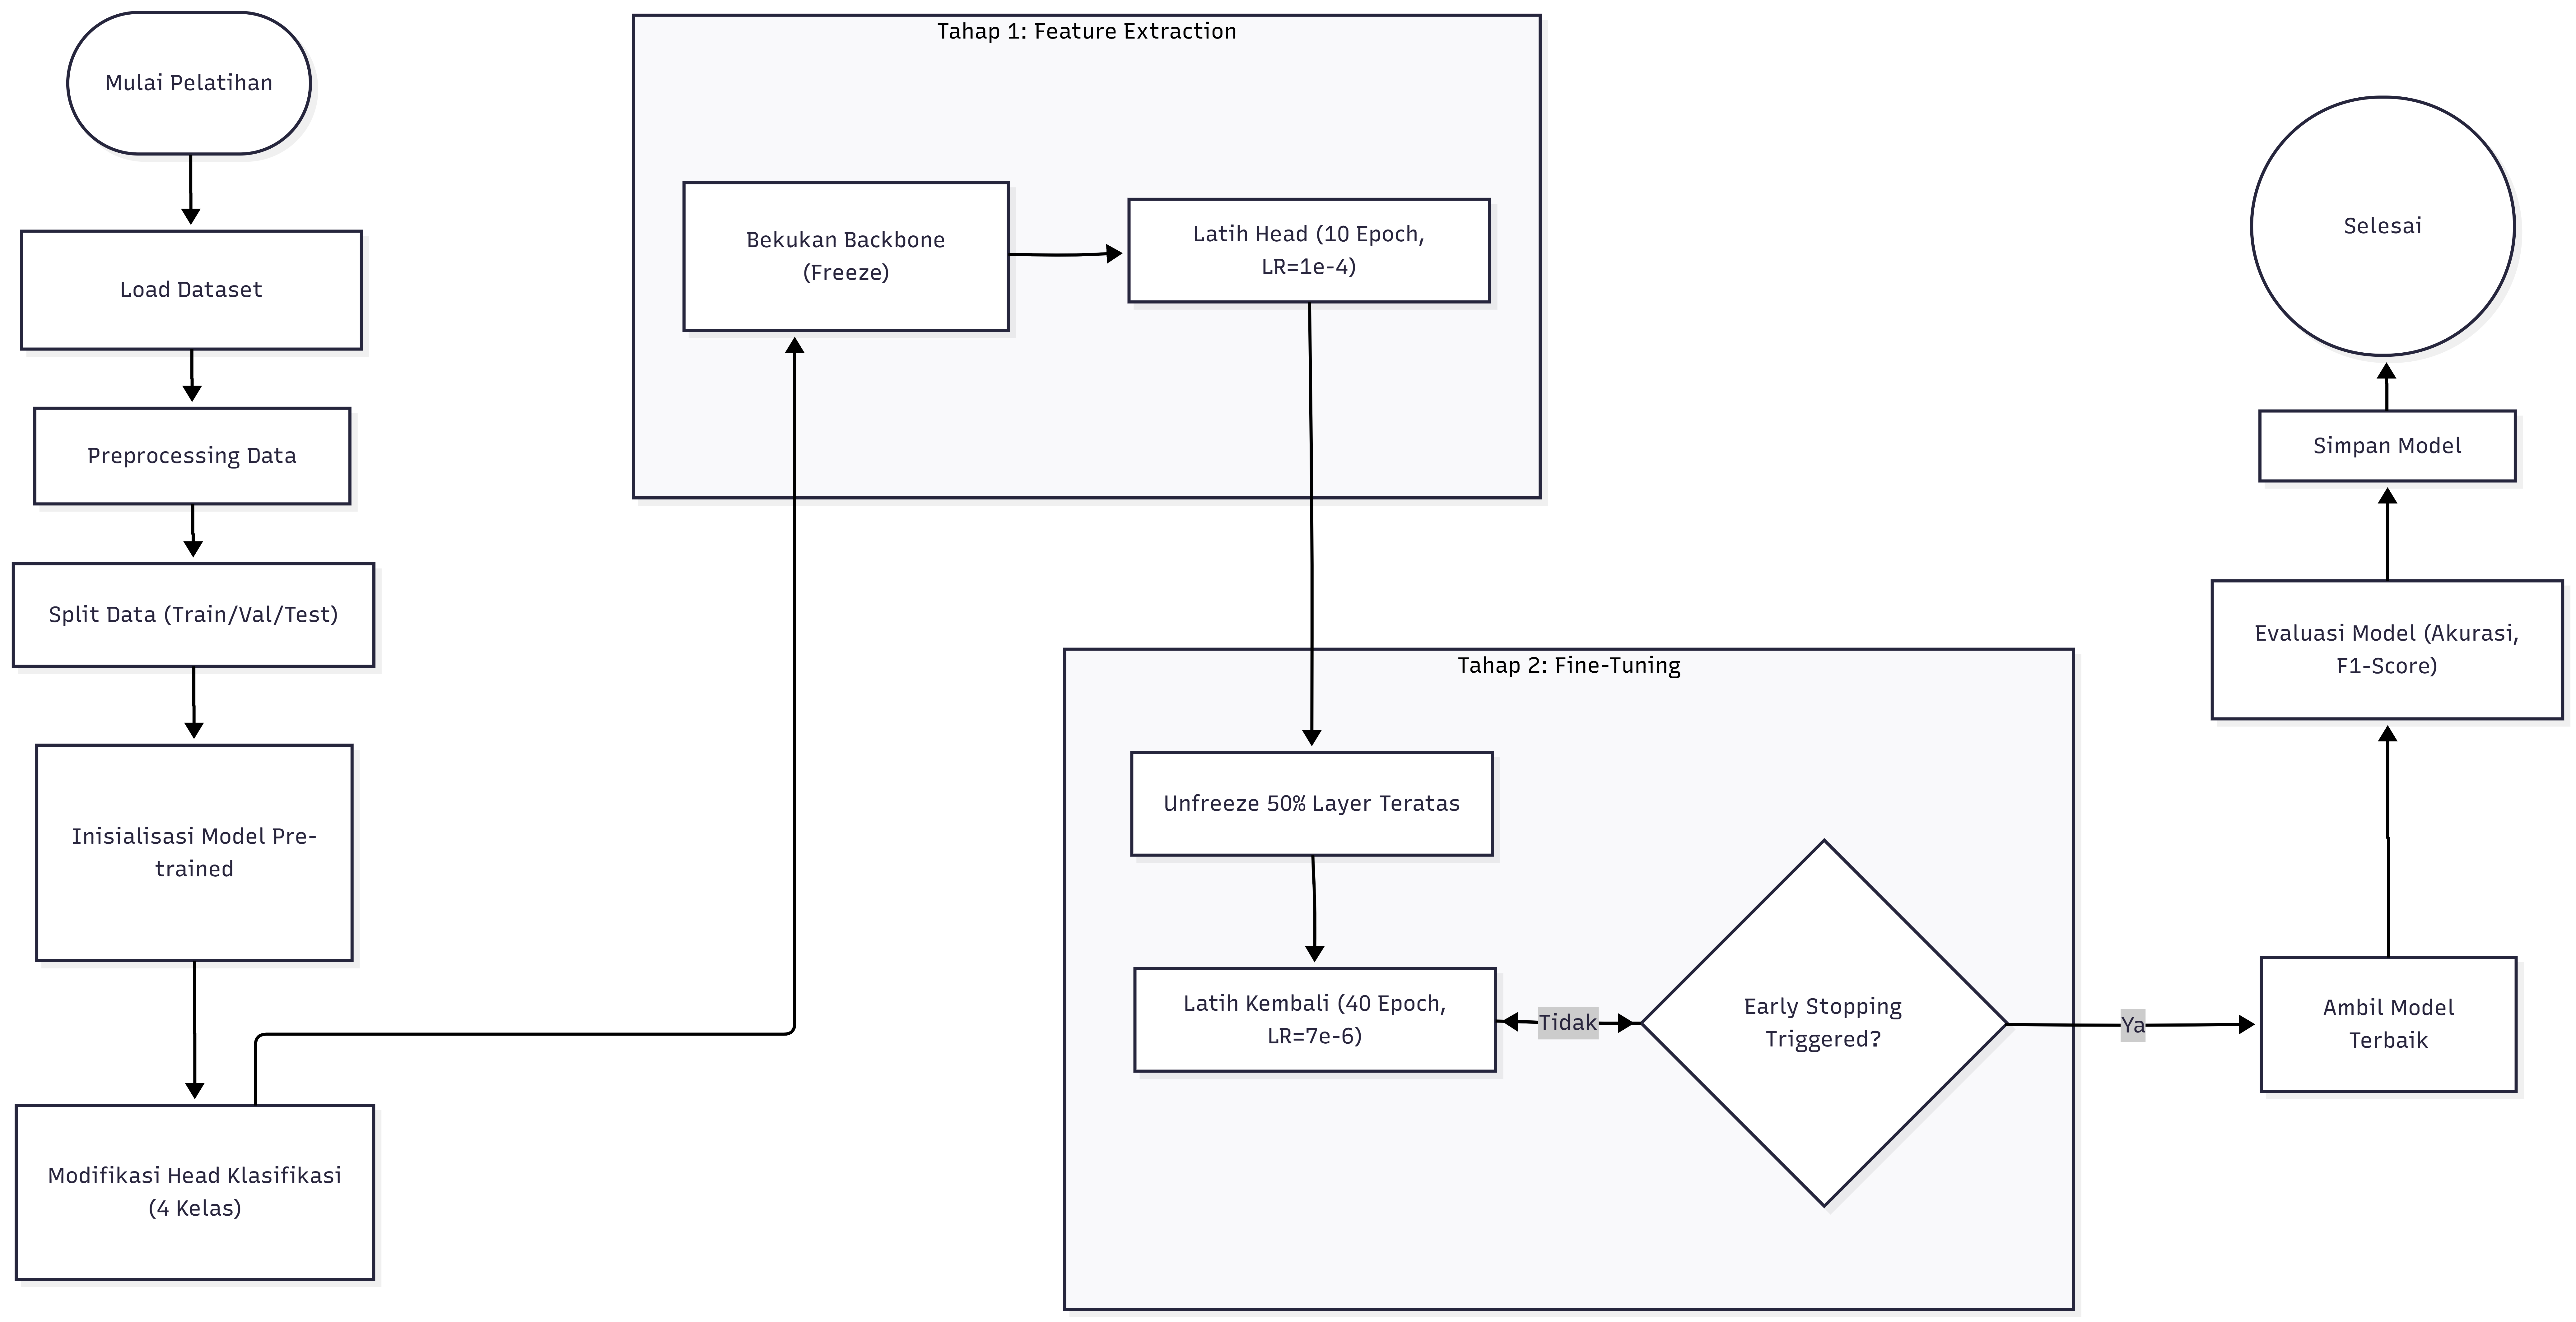
\includegraphics[width=\linewidth]{gambar/flowchart-klasifikasi.png}
	\caption{Diagram Alur Modul Klasifikasi}
	\label{fig:flowchart-klasifikasi}
\end{figure}

Desain modul klasifikasi ini mengeksplorasi dua arsitektur \textit{deep learning} untuk tugas \textit{computer vision}, yaitu \textit{Convolutional Neural Network} (CNN) menggunakan model ResNet, DenseNet, dan EfficientNet serta arsitektur Transformer menggunakan \textit{Vision Transformer} (ViT) dan Swin Transformer. Lapisan akhir setiap model dimodifikasi menjadi \textit{classification head} untuk menghasilkan probabilitas bagi empat kelas target.

\subsection{Desain Modul Koreksi Citra}

Modul koreksi dirancang untuk tugas translasi gambar ke gambar (\textit{image-to-image translation}). Arsitektur yang digunakan adalah Pix2Pix \textit{Conditional GAN} untuk merekonstruksi gambar bersih dari gambar dengan artefak. Arsitektur modul koreksi dapat dilihat pada Gambar \ref{fig:flowchart-koreksi}. 

\begin{figure}[H]
	\centering
	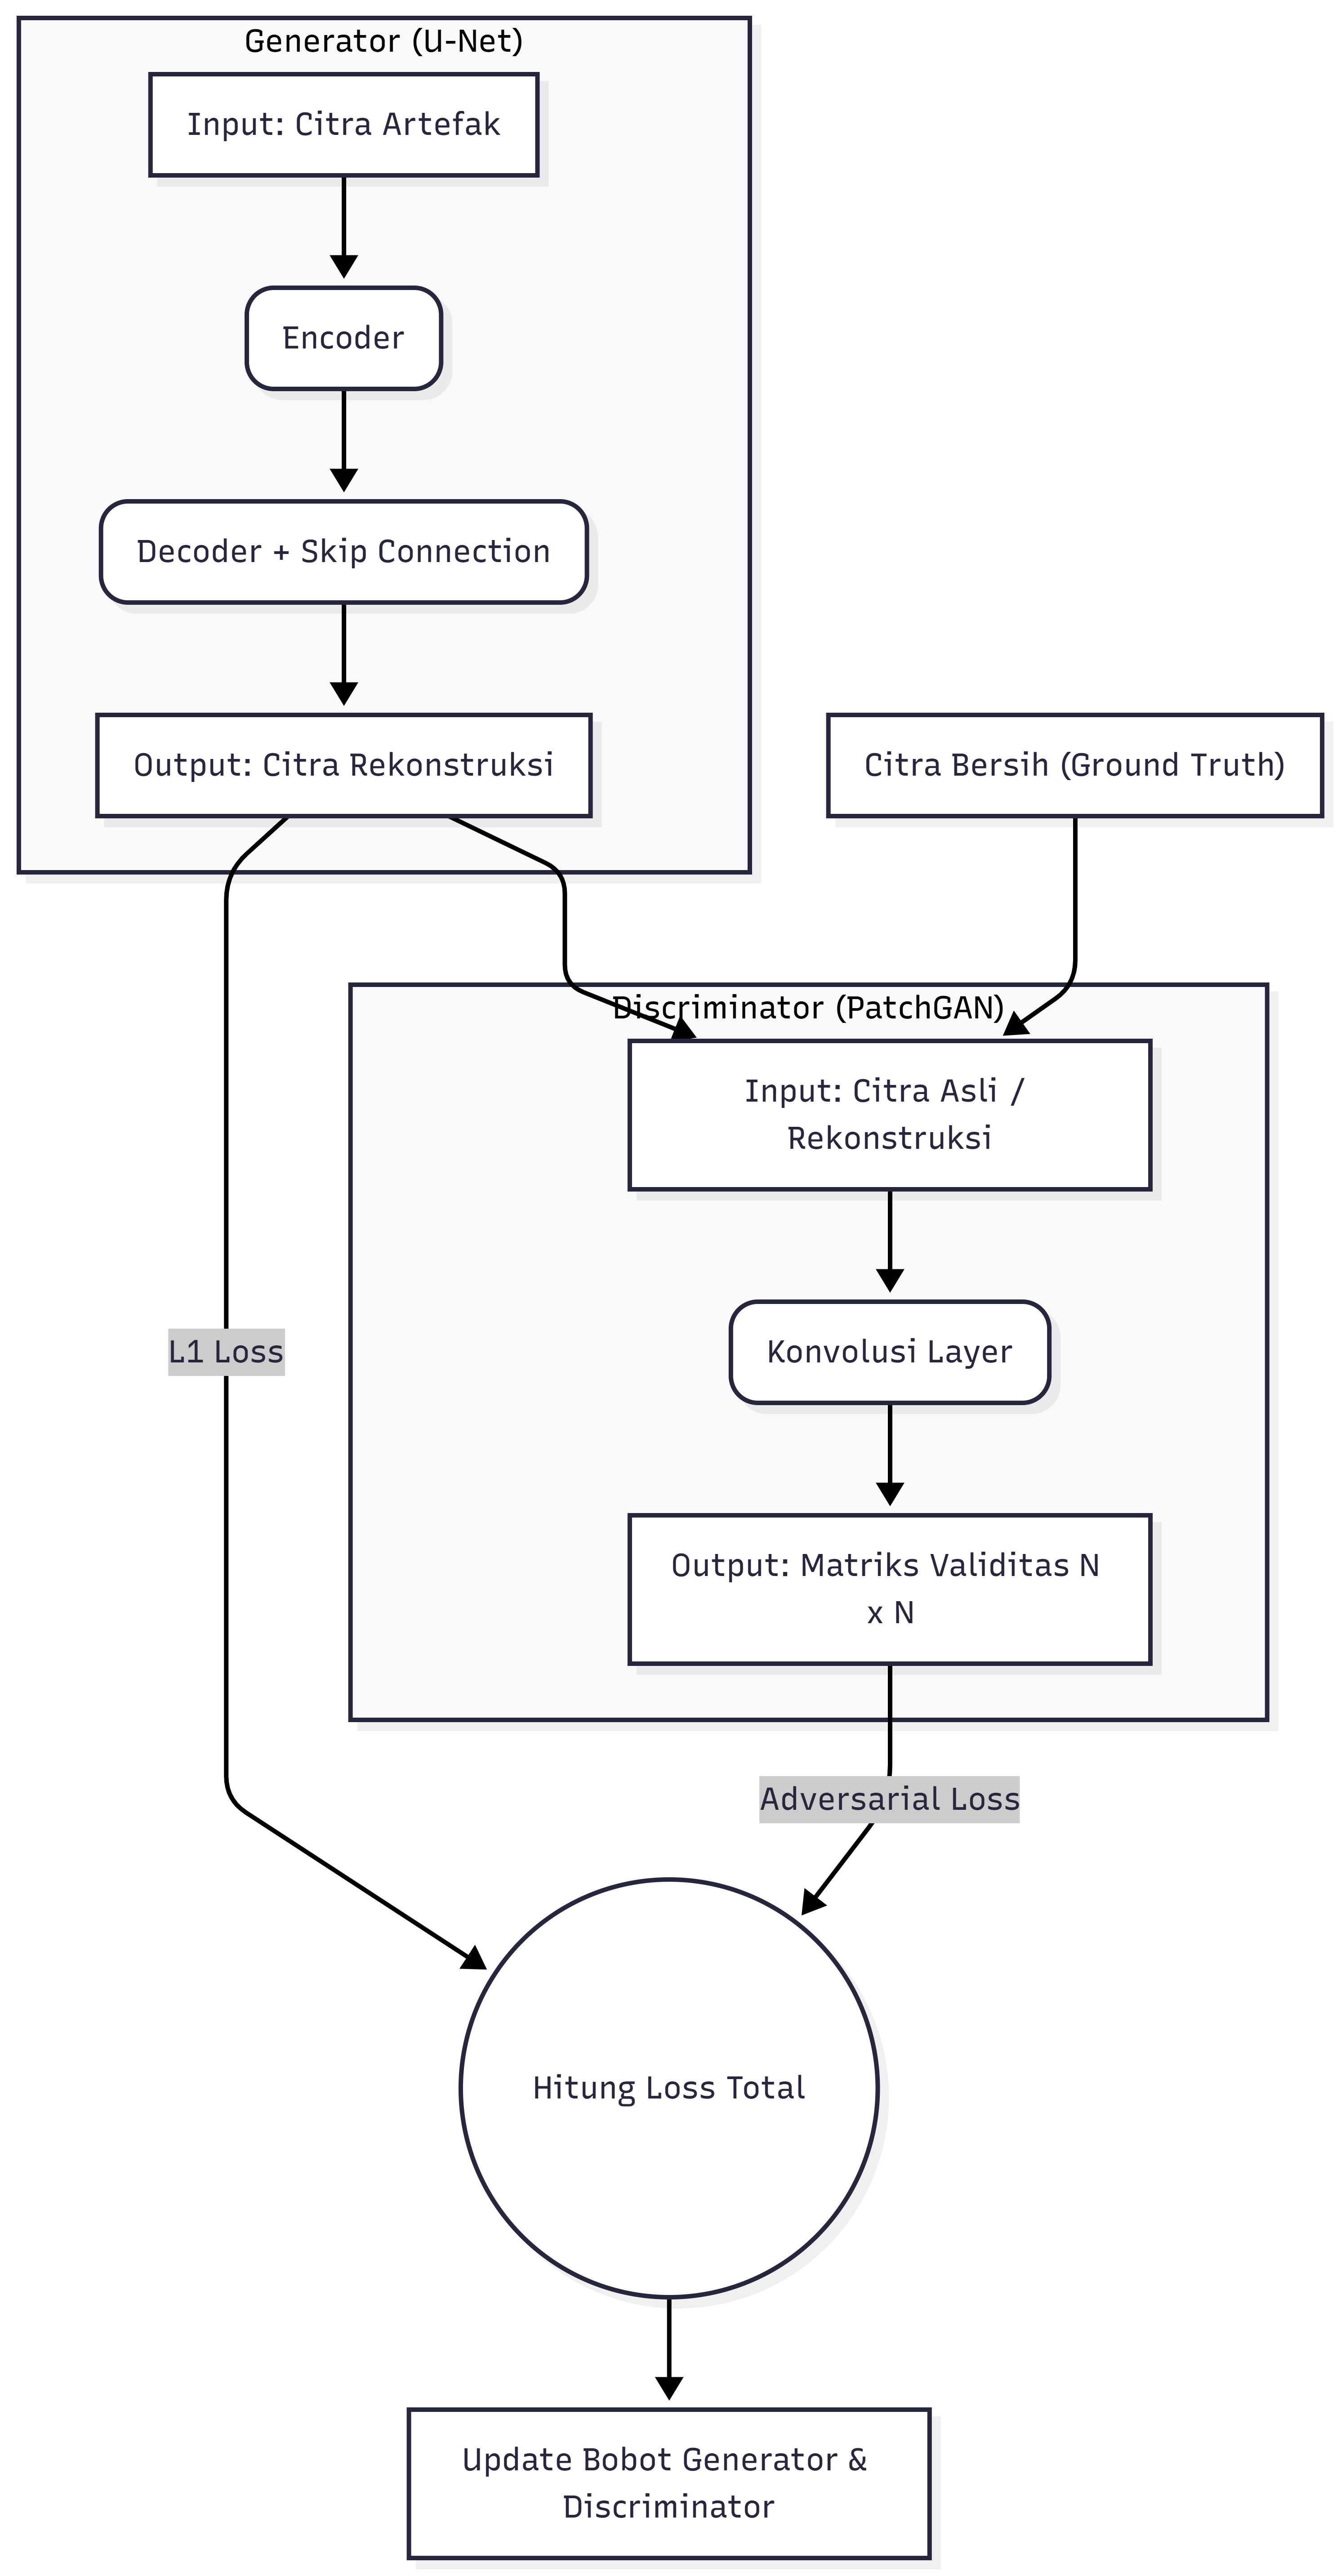
\includegraphics[width=0.5\linewidth]{gambar/flowchart-koreksi.png}
	\caption{Diagram Alur Modul Koreksi Citra}
	\label{fig:flowchart-koreksi}
\end{figure}

Pix2Pix terdiri dari dua komponen yang saling berkompetisi:

\begin{enumerate}[nolistsep]
	\item \textit{Generator} berbasis U-Net yang bertugas menerima input citra dengan artefak dan menghasilkan citra bersih. Arsitektur U-Net digunakan karena adanya \textit{skip connections} yang memungkinkan informasi detail struktur otak dari input tetap terjaga hingga \textit{output}.
	
	\item \textit{Discriminator} berbasis \textit{convolutional PatchGAN} yang bertugas membedakan antara citra bersih asli dan citra hasil rekonstruksi \textit{Generator}. PatchGAN bekerja dengan menilai realisme citra pada level \textit{patch} lokal yang efektif untuk menghasilkan tekstur yang tajam.
\end{enumerate}

\section{Implementasi Sistem}

\subsection{Implementasi Pembuatan Dataset}

\subsection{Implementasi Modul Klasifikasi}

\subsection{Implementasi Modul Koreksi Citra}
Alat diimplementasikan dengan \lipsum[22]

% Contoh pembuatan code snippet
\begin{lstlisting}[
  language=C++,
  label={lst:Hello World},
  caption={Program hello world}
]
#include <iostream>

int main() {
    std::cout << "Hello World!";
    return 0;
}
\end{lstlisting}

% Contoh penggunaan referensi dari code snippet yang diinputkan
Seperti contoh pada baris program Listing \ref{lst:Hello World} dan Listing \ref{lst:PrimeNumber}, \lipsum[23]

% Contoh input code snippet
\lstinputlisting[
  % Bahasa yang digunakan oleh code snippet
  language=Python,
  % Label referensi dari code snippet yang diinputkan
  label={lst:PrimeNumber},
  % Keterangan dari code snippet yang diinputkan
  caption={Program perhitungan bilangan prima}
% Nama dari file code snippet yang diinputkan
]{program/prime-number.py}
